\documentclass{article}
\usepackage[utf8]{inputenc}
\usepackage{graphicx}
\usepackage{fancyhdr}
\usepackage{verbatim}
\usepackage[danish]{babel}
\pagestyle{fancyplain}
\author{Mikkel Kragh Mathiesen, Jannik Gram, Rune \& Rasmus Abrahams{\tt (son|en)}}
\title{}
\date{\today}
\lhead{Mikkel, Jannik, Rune \& Rasmus}
\rhead{\today}
\begin{document}

\maketitle

\section{Analyse af modellerings- og simuleringsprocesser}
\subsection*{(1.a)}
Artiklen indeholder modellerne ``matematisk model'' og ``diskret model''; den indeholder processerne ``idealisering'' og ``diskretisering''.

Den matematiske model består af ligninger.

Artiklen præsenterer problemstillinger fra den virkelige verden omhandlende udfordringen med at afgøre hvordan de forskellige led på en robot eller et menneske skal bevæge sig for at opnå forskellige mål. Dette hører ind under boksen ``Real World''. Med dette i mente opstilles der en model under en proces, der retteligt kan betegnes som idealisering. Den resulterende model er matematisk af karakter og hører ind under boksen af samme navn. Til sidst ligger den matematiske model grund til udformningen af en algoritme, der hører ind under boksen ``diskret model''. Dette udgør processen ``diskretisering''.

Artiklen verificerer ikke den diskrete model. Der er flere måder på hvilke dette kunne gøres. En mulig måde er formel verifikation af algoritmen ved brug af for eksempel Hoare-logik, men det praktiske aspekt af dette kan muligvis være for omfattende. En anden mulighed er et udføre dækkende afprøvninger.

verification
simulation
results
validation

\section{Boldsimulator}

\section{Kantfinder}

\subsection*{(3.a)}

\begin{figure}
	\begin{verbatim}
		function r = sobel_fold(A, B)
		    r = 0;
		    for i=1:3
		        for j=1:3
		            r = r + A(i,j)*B(i,j);
		        end
		    end
		end
	\end{verbatim}
	\caption{Kildekode til sobel\_fold.m}
	\label{sobelfold}
\end{figure}

\begin{figure}
	\begin{verbatim}
		function J = edge_detector(I)

		[M, N] = size(I);
		J = zeros( size(I) );

		Ex = [-1 -2 -1; 0 0 0; 1 2 1];
		Ey = [-1 0 1; -2 0 2; -1 0 1];

		for i=2:M-1
		  for j=2:N-1

		    A = zeros(3);

		    A(1,1) = I(i-1,j-1);
		    A(1,2) = I(i-1,j  );
		    A(1,3) = I(i-1,j+1);

		    A(2,1) = I(i  ,j-1);
		    A(2,2) = I(i  ,j  );
		    A(2,3) = I(i  ,j+1);

		    A(3,1) = I(i+1,j-1);
		    A(3,2) = I(i+1,j  );
		    A(3,3) = I(i+1,j+1);

		    val1 = sobel_fold(A, Ex);
		    val2 = sobel_fold(A, Ey);
		    J(i,j) = sqrt( val1^2 + val2^2 );
		  end
		end

		end
	\end{verbatim}
	\caption{Kildekode til edge\_detector.m}
	\label{edgedetector}
\end{figure}

Sobeloperationen er implementeret i funktionen på figur~\ref{sobelfold} og bruges i {\tt edge\_detector} på figur~\ref{edgedetector}.

Bemærk at koden ikke tager højde for problemer i forbindelse med gitterets yderste pixels. Således har en kantpixel forholdsmæssigt op til tre færre naboer at sammenligne sig med. Konsekvenserne af dette kan for eksempel ses på figur~\ref{bla} og figur~\ref{bla'}, hvor de to sorte linier mod forventning ikke helt når billedrammen.

\subsection*{(3.b)}

Vi har tænkt os at udsætte kant-finderen for et 
	basistilfælde, for at se om den virker. Dette vil gøres
	med et meget simpelt billede med et par sorte streger
	på hvid baggrund, så man tydeligt kan se om den farver
	de rigtige kanter, som i dette tilfælde er stregerne.
	Derudover vil vi også teste særtilfælde med billeder 
	uden kanter og billeder, der har færre end 3 pixels
	i hver dimension. Vi vil også teste meget store 
	billeder for at se om programmet også kan håndtere
	disse.
	\begin{figure}
		\centering
		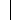
\includegraphics[width=3in]{test1.png}
		\caption{Billede}
		\label{ke1}
	\end{figure}
	\begin{figure}
		\centering
		
\includegraphics[width=4in]{test1_result.png}
		\caption{Resultat}
		\label{ke1r}
	\end{figure}
	\begin{figure}
		\centering
		
\includegraphics[width=3in]{test2.png}
		\caption{Billede}
		\label{ke2}
	\end{figure}
	\begin{figure}
		\centering
		
\includegraphics[width=4in]{test2_result.png}
		\caption{Resultat}
		\label{ke2r}
	\end{figure}
	\begin{figure}
		\centering
		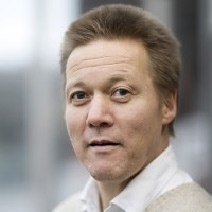
\includegraphics[width=3in]{test3.jpg}
		\caption{Billede}
		\label{ke3}
	\end{figure}
	\begin{figure}
		\centering
		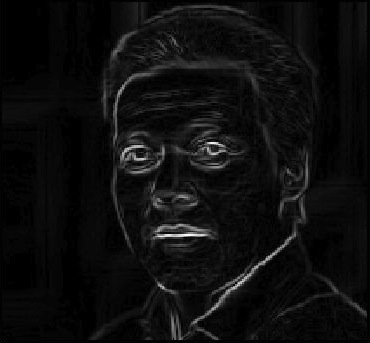
\includegraphics[width=4in]{test3_result.jpg}
		\caption{Resultat}
		\label{ke3r}
	\end{figure}

\end{document}
